\documentclass[11pt,a4paper]{article}
\usepackage{od,amsmath,wrapfig}
\usepackage[utf8]{inputenc}
\usepackage[russian]{babel}

\title{ТРИЗ как метод анализа и создания экологичных\\ и устойчивых
  технологических систем} 

\author{Дитрих Бальцер, Вернер Реген, Фридер Зибер}
\date{2018}

\begin{document}
\maketitle

\section*{1. Введение}
\begin{wrapfigure}[19]{l}{.25\textwidth}\vspace*{-1em}
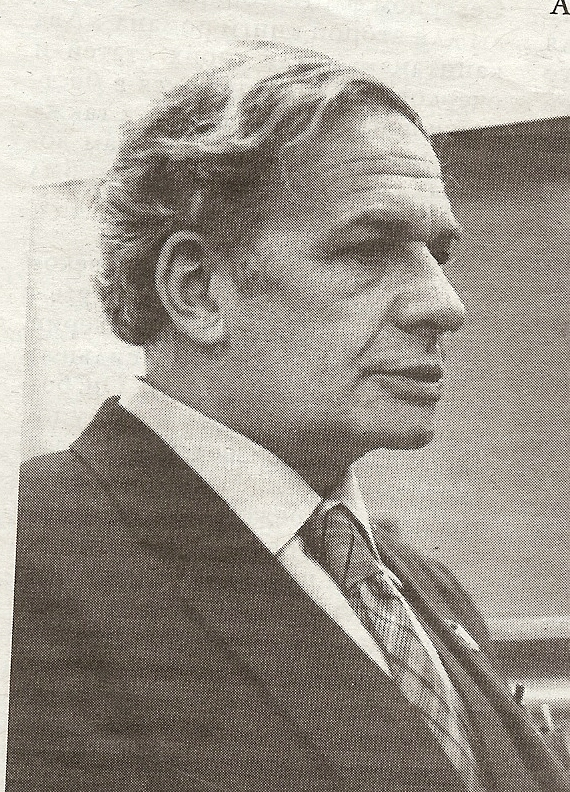
\includegraphics[width=.25\textwidth]{qvViZa.jpg}
\caption{Генрих Саулович Альтшуллер (1926--1998)}
\end{wrapfigure}
Теория решения изобретательских задач (ТРИЗ), созданная советским ученым
Генрихом Сауловичем Альтшуллером (Рис. 1), приобретает все большую
известность. Этот метод используется по всему миру, например, в Европе и в
США, а также в Китае и в Корее [1,2,3].

В данной статье подводятся итоги и обобщается опыт при использовании методов
ТРИЗ в рамках междисциплинарных исследований по проблемам окружающей среды в
промышленности Германии. Авторы статьи являются членами Института
междисциплинарных исследований\footnote{LIFIS, Leibniz-Institut für
  interdisziplinäre Studien, \url{https://www.leibniz-institut.de}.}, как
составной части научного общества имени Лейбница\footnote{Leibniz-Sozietät der
  Wissenschaften, \url{https://www.leibnizsozietaet.de}.}. Данный институт
имеет следующий профиль:
\begin{itemize}
\item координация научных исследований, проводимых по разным направлениям
  естественных, технических и общественных наук;
\item распространение научных знаний;
\item укрепление связей между наукой и учебой.
\end{itemize}
Одна из основных целей научно-технической деятельности LIFIS – улучшение
экологических показателей производства. Кроме этого LIFIS занимается
распространением методов ТРИЗ в составе интердисциплинарного инновационного
менеджмента.

В данной статье рассматриваются следующие проблемы:
\begin{itemize}
\item характеристика современной ТРИЗ;
\item междисциплинарные исследования (ТРИЗ, непрерывная технология,
  искусственный интеллект, кибернетика) и их практическая реализация в рамках
  научно-технических проектов;
\item содержание учебной деятельности по интердисциплинарному инновационному
  менеджменту, включая ТРИЗ.
\end{itemize}
\section*{2. Современная ТРИЗ}
Классическая ТРИЗ является общетехнической версией. Для практического
использования в технике необходимо иметь множество специализированных версий
ТРИЗ, отличающихся между собой номенклатурой и содержанием. Между различными
версиями ТРИЗ, безусловно, существуют аналогии. Некоторые крупные корпорации
уже применяют специализированные версии ТРИЗ, адаптированные к своим областям
деятельности. Так, например, промышленные предприятия бизнес-группы «Базовый
Элемент» (\url{www.basel.ru}) реализуют масштабные инновационные проекты в
сотрудничестве с ведущими российскими и международными инжиниринговыми
компаниями, вузами и научно-исследовательскими институтами. При этом
применяются специализированные версии ТРИЗ, направленные на повышение
эффективности операционной деятельности за счет автоматизации деятельности с
целью снижения энергопотребления, повышения производительности оборудования и
минимизации отходов.

Данная статья посвященa разработке версии ТРИЗ для синтеза и эксплуатации
непрерывных технологических процессов. Эти процессы играют центральную роль в
экологической сфере.

Современная ТРИЗ ориентирована во-первых на \textbf{междисциплинарность} при
решении диалектических противоречий и во-вторых на системный и комплексный
подход к реализации \textbf{стратегии устойчивого развития} [4].

Стратегия устойчивого развития (англ.: Sustainability, нем.: Nachhaltigkeit)
впервые была сформулирована саксонским обер-берггауптманом Хансом Карлом фон
Карловицем (Рис. 2).

\begin{wrapfigure}{l}{.25\textwidth}\vspace*{-1em}
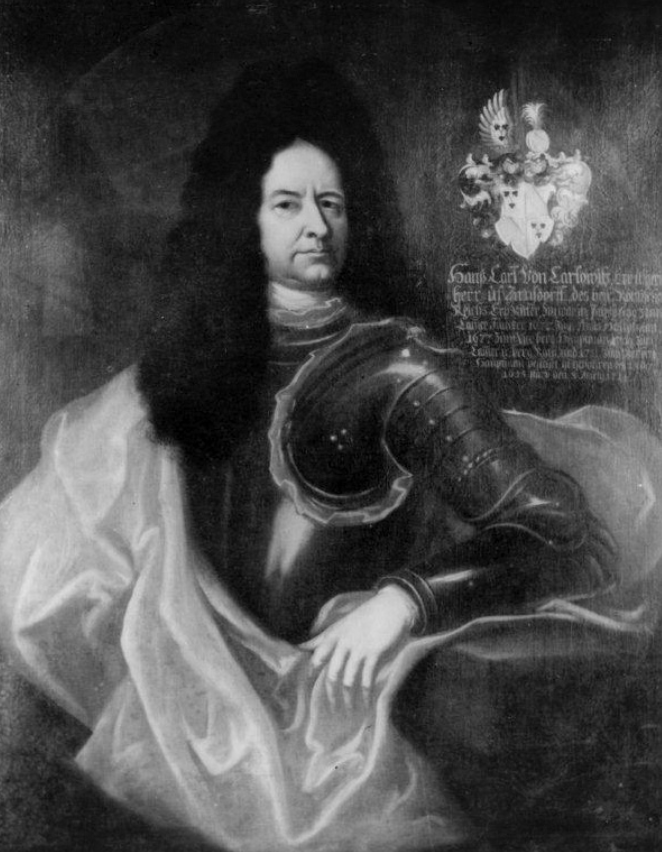
\includegraphics[width=.25\textwidth]{oQWNOq.png}
\caption{Ханс Карл фон Карловиц (1645--1714)} 
\end{wrapfigure}
В связи с развитием горнодобывающей промышленности, которая требовала для
получения разных металлов большое количество древесины, он применял эту
стратегию для разработки концепции по устойчивому развитию лесного хозяйства в
Саксонии. В своей книге  «Sylvicultura oeconomica ...» [5], опубликованной в
Лейпциге в 1713 году, он сформулировал правило устойчивого развития лесного
хозяйства:  «Разрешается потреблять столько древесины, сколько растет!»  Три
основных компонента или аспекта устойчивого развития можно представить в виде
«треугольника устойчивости» (рис.3).
\begin{figure}[h]
  \begin{center}
    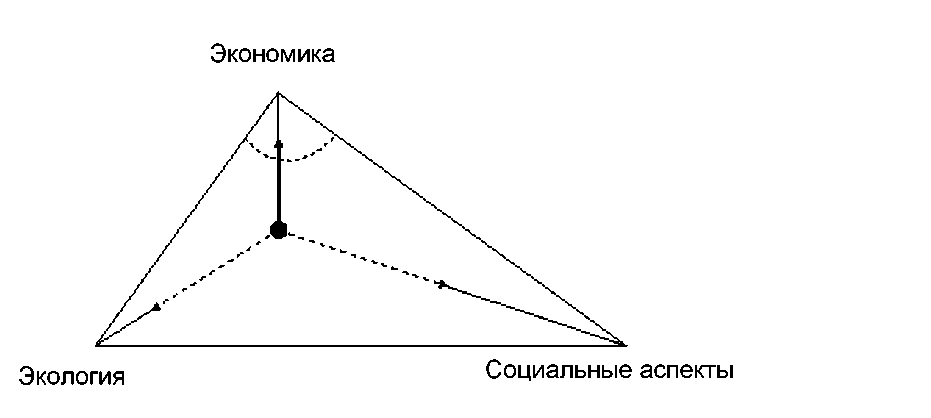
\includegraphics[width=.75\textwidth]{a7McJu.png}
    \caption{Треугольник устойчивого развития [6]} 
  \end{center}  
\end{figure}
Фокус треугольника в настоящее время все еще находится в пунктирной области
«экономики». Необходимо смещать фокус в направлении “экологии” и  «социальных»
аспектов, чтобы он, на самом деле, находился около центра. Тогда все три
аспекта будут одинаково учтены. Важно ускорить этот процесс “смещения фокуса”.
«Управляющим воздействием» в этом процессе являются структура и параметры
технологических систем (установки, включая системы автоматизации). Рабочая
группа  «Общая технология» научного общества имени Лейбница регулярно проводит
симпозиумы на тему  «Технология и устойчивое развитие» (см. напр. [7]).
Результаты этих симпозиумов вошли в данную статью.

При разработке и эксплуатации непрерывных технологических процессов можно выделить 3 вида диалектических противоречий:
\begin{itemize}
\item административное противоречие: Противоречие между идеей и реальностью;
\item противоречие с точки зрения технических наук: Типичными примерами
  являются противоречие между заданием регуляторам и фактическим значением
  параметров процесса и противоречие между оптимальностью и устойчивостью
  (стабильностью) процесса;
\item противоречие с точки зрения естественных наук (химия, физика, биология и
  др.): Это противоречие является наиболее фундаментальным, потому что
  изобретатель упирается в ограничения, обусловленные законами природы,
  например: Зaкон Бойля-Мариотта, Закон Ома.
\end{itemize}
Существует большое количество приёмов для устранения или решения этих
противоречий, например: Введение обратной связи, разложение всей системы на
подсистемы, универсальность за счет использования количественных
фундаментальных знаний (математических моделей). На примере получения
углеводородов из органических отходов ниже будет показано, как применяется
выше описанный подход.

Когда мы говорим о стратегии устойчивого развития мы должны учитывать
технические, экономические, экологические и социальные проблемы. В смысле
устойчивости необходимо решить задачу поликритериальной оптимизации (векторная
оптимизация). Речь идет об определении множества Парето по экономическим,
экологическим и социальным критериям.  «Управляющим воздействием» при
определении множества Парето являются структура и параметры технологической
установки (объект управления) и её системы автоматизации. Структура и
параметры системы автоматизации выбираются так, чтобы при автоматическом
управлении (автоматическая оптимизация, стабилизация и защита) были выполнены
условия оптимальности и устойчивости. При этом речь идет прежде всего об
адаптивных решениях с использованием элементов искусственного интеллекта в
режиме реального времени и, во-вторых, о повторном использовании отдельных
элементов cистем автоматизации.

В настоящее время автоматизация может рассматриваться как ключ к устойчивым технологическим процессам или к устойчивому развитию. Вместо термина  «Автоматизация» часто применяются понятия  «Производство 4.0»,  «Цифровая экономика» или  «Дигитализация».
Под экономическим критерием мы понимаем конкурентоспособность реализованных
технологических систем, под экологическим критерием - эффективность
использования ресурсов и энергии, и под социальным критерием - физиологические
и психологические условия работы. В данном случае необходимо отметить, что в
других версиях ТРИЗ социальный критерий может иметь более широкий смыл.

Являясь интеграционной научной дисциплиной, автоматизация имеет все
предпосылки для решения этой поликритериальной задачи.
\end{document}

3. Междисциплинарные исследования (ТРИЗ, непрерывная технология, искусственный интеллект, кибернетика)

Междисциплинарные исследования используя ТРИЗ, искусственный интеллект и кибернетику требует сравнительного анализа этих научных дисциплин [8]. В то время как для ТРИЗ, искусственного интеллекта и кибернетики общей характерной особенностью является комплексное использование накопленного человеческого знания существуют однако значительные отличия между ними, как показано в таблице 1.

 
Содержание процесса решения
Динамика процесса решения
Техническая реализация
ТРИЗ 
Противоречия как диалектический принцип, большое количество инновационных базовых приёмов (разложение, интеграция, обратная связь и т.д.)
Нет возможности работы в режиме реального времени
Автоматизированное автономное решение с целью изобретения (CAI)
Искусственный интеллект 
Феноменологическое (экспертные и фасси-системы) и биологические (нейронные сети) описание человеческого мыслительного процесса 
Работа в режиме реального времени возможна
Может быть интегрирован в системы автоматизации и управления с целью оптимизации системы, тесная связь с технической кибернетикой
Кибернетика
Сбор, обработка и использование информации, онлайн-соединение с объектом управления
Работа в режиме реального времени возможна и абсолютно необходима
Автоматизированные системы управления технологическими процессами (АСУТП), использование виртуальных сетей автоматизации

Таб. 1: Сравнение ТРИЗ, искусственного интеллекта и кибернетики

Ясно, что обмен информацией и опытом между представителями трех названных дисциплин может принести пользу всем. Эта статья призвана стать практическим шагом в этом направлении. Дальше рассматриваются следующие вопросы:
    • Предмет кибернетики и искусственного интеллекта с точки зрения сотрудничества с ТРИЗ;
    • Практические примеры технических систем, деятельность которых может быть улучшена с помощью ТРИЗ;
    • Методология математического моделирования для извлечения фундаментальных знаний;
    • Взаимная польза от сотрудничества ТРИЗ, искусственного интеллекта и кибернетики.

3.1 Предмет кибернетики и искусственного интеллекта с точки зрения сотрудничества с ТРИЗ

Задачи кибернетики приведены в таблице 2.

Функции управления
Объяснение функции управления 
Типовые технические решения
Защита процессов
Сигнализация, аварийный останов в случае опасных ситуаций, реализация защитных стратегий, предотвращение неисправной работы оператора
Защитные системы блокировки, управление процессами останова, интеллектуальная превентивная защита процессов
Стабилизация процессов
Автоматическая компенсация возмущений, динамическая развязка подсистем 
Системы регулирования, интеллектуальная координация процессов
Оптимизация процессов
Определение и настройка оптимальных режимов работы, определение и реализация оптимальных переходных процессов (переключение, запуск и т.д.)
Использование алгоритмов оптимизации

Таб. 2: Функции управления как задачи кибернетики 

Методы кибернетики основаны на единице системы управления и объекта управления. По этой причине задачи системы управления определяются сравнительным анализом амплитуды и частоты возмущений, действующих на управляемый объект (см. рис. 4). 






















Рис. 4: Определение задач управления

Кроме того, на рисунке 4 показано, что с уменьшением частоты возмущений рекомендуется использование искусственного интеллекта (экспертные системы). То же самое относится и к применению методов ТРИЗ к использованию человека в качестве регулятора (открытый контур).
Рассматривая методы искусственного интеллекта, мы полагаем, что в первую очередь используются экспертные системы, способные к управлению процессами в режиме реального масштаба времени. Базовая структура таких экспертных систем существует уже с 1992 и показана на рисунке 5 [9].





















Рис. 5: Экспертные системы реального времени для решения задач управления

Разработчиком и пользователем экспертных систем часто является одно и то же лицо.
В таблице 3 описаны функции компонентов экспертных систем, показанных на рисунке 5.

Компоненты
Функции
Объяснение 
База знаний
Представление знаний
Содержит специфичное для применения знание
Компонент решения проблем
Манипулирование знаниями
Основывается на теориях и стратегиях для решения задач определенных классов проблем
Компонент сбора знаний
Приобретение знаний
Помогает эксперту при синтезе баз знаний
Пояснительный компонент
Объяснение содержания знаний
Объясняет разработчику или пользователю путь решения
Компонент диалога
Обмен знаниями
Общается с разработчиком или с пользователем

Таблица 3: Функции компонентов экспертных систем  

Данные о технологических процессах, собираемые в режиме онлайн с целью управления технологической установкой, передаются в базу знаний в качестве специфического знания конкретных случаев. Специфические знания, используемые в экспертных системах, имеют следующие формы знаний:
- ассоциативные или эмпирические знания как логическая связь между технологическими характеристиками и выводами в виде правил (симптомы-ситуации, ситуации-управляющие воздействия, управляющие воздействия-эффекты или результаты);
- качественные фундаментальные знания как модели, описывающие структуру (абстракция, агрегация, связь, подход) и функции (причинно-следственные цепи, штатный режим, аварийная ситуация) объекта управления и системы управления;
- количественные фундаментальные знания как аналитические модели системы (математические модели, использующие законы естествознания для описания статических и динамических свойств технических систем).

Эти формы знаний играют важную роль в сотрудничестве с методами ТРИЗ.
В то время как ассоциативные или эмпирические знания обычно вытекают из опыта оператора при эксплуатации установки завода, фундаментальные знания являются результатом глубокого научного анализа установки.
Примером ассоциативных знаний по отношению к управлению установкой по получению углеводородов из органических отходов (см. 3.2) является:

Если температура в турбо-реактор выше, чем 250 градусов цельсия,
Тогда снизить скорость вращения лопастей и уменьшить подачу кислорода.
На рисунке 6 показана структура системы, состоящей из 3 подсистем, как пример качественных фундаментальных знаний.















Рис. 6: Cистема, состоящая из 3 подсистем 
- вектор возмущений, - вектор управляющих воздействий,
 - вектор выходных величин

В разделе 3.2 приводятся примеры количественных фундаментальных знаний, также применительно к установке по получению дизеля из органических отходов.
В таблице 4 описываются преимущства и недостатки различных форм знаний.

Формы знаний 
Преимущства 
Недостатки 
Ассоциативные или эмпирические знания 
 Интеграция опыта (простое моделирование), среднее вычислительное усилие (хорошая способность к работе в реальном времени), эксплицитные знания (правила, понятное содержание)
Более высокая специализация (ограниченное повторное использование), необходимо записать всю информацию (полнота не гарантирована)
Качественные фундаментальные знания 
Более высокая универсальность (возможно повторное использование решений),
Обнаружение непредвиденных случаев (полнота),
Эксплицитное и понятное знание 
Высокие вычислительные затраты (ограниченные возможности относительно режима реального времени),
Презентация только простых контекстов (ограниченная конфигурируемость контекстов)
Количественные фундаментальные знания 
Представление сложных корреляций (применение математических моделей, вывод правил), подходит для моделирования, планирования и управления (высокая адекватность моделей)
Большие вычислительные затраты (ограниченные возможности относительно режима реального времени), сложности при объяснении знания

Таб. 4: Преимущства и недостатки различных форм знаний

Важно сравнить структурирование и обработку знаний при ТРИЗ, искусственном интеллекте и кибернетике для проектирования интерфейса между программными пакетами этих 3 дисциплин (см. таблицу 5).

 
Структура знаний, 
Манипуляция знаниями
ТРИЗ
Таблицы противоречий, инновационные принципы или приёмы (около 40) для решении противоречий
Логика, структурный анализ, CAI
Искусственный интеллект/ кибернетика
Ассоциативные или эмпирические знания (правила), качественные и количественные фундаментальные знания (процедурные и математические модели)
Логика, оболочки экспертных систем  

Таблица 5: Презентация и обработка знаний при ТРИЗ, искусственном интеллекте и кибернетике

3.2 Получение углеводородов из органических отходов  

Целью данного технологического процесса является то, чтобы ранее неиспользуемые органические отходы превратить в углеводороды, которые затем используются в качестве топлива или сырья в химической и другой промышленности [8].    

Разные установки по производству углеводородов из органических отходов должны быть интегрированы в виртуальную электростанцию (Micro Grid). Это значит, что генерируемая из углеводородного топлива локально на ТЭЦ энергия (электрическая и тепловая) используется на месте. Дорогих линий передачи электрического тока больше нет. В то же время затраты на транспортировку исходных материалов резко снижаются по сравнению с центральными производителями энергии.

Технологическая схема получения углеводородов из органических отходов показана на рисунке 7.



























Рис. 7: Технологическая схема получения углеводородов из органических отходов  

Центральными элементами технологической установки являются турбина (турбо-реактор) для производства углеводородного топлива, сепаратор и колонна дистилляции для отделения дизельного топлива от других углеводородов (см. рис. 8).


















Рис. 8: Внешний вид технологической установки в Бранд-Эрбисдорфе (Саксония, Германия)

В турбине с инъекцией кислорода (рис. 9) протекают трибохимические реакции деполимеризации и полимеризации в присутствии минерального катализатора.
















Рис. 9: Турбина с инъекцией кислорода
При этом получается дизель.
Основными характеристиками технологического процесса являются:
    • низкие температуры и нормальное давление;
    • отсутствие образования диоксинов (охрана окружающей среды);
    • исходными материалами являются биогенные отходы (солома, древесина и др.), а также такие высококалорийные отходы как пластмассы. 
Чтобы интегрировать локальные ТЭЦ и установки по производству углеводородного топлива в виртуальную электростанцию, надо решить следующие проблемы:
- повысить производительность системы;
- для генерации управляющей энергии в виртуальной электростанции необходимо обеспечить широкие диапазоны изменения параметров производительности;
- необходимо иметь возможность значительного изменения скорости произведенного количества топлива в единицу времени;
- иметь достаточно низкую инерционность системы.

Для решения этих проблем были использованы методы ТРИЗ в сочетании с методами искусственного интеллекта и кибернетики.
В ходе процесса решения были рассмотрены следующие диалектические противоречия:
Противоречие между номинальной или заданной величиной параметров процесса и фактическим значением параметров процесса при эксплуатации технологических систем является характерным диалектическим противоречием при управлении непрерывными технологическими процессами. Конечно, это также относится к процессам получения дизеля из органических отходов.  
Заданное значение является зависимой от времени функцией, которая служит заданием регуляторам. В нашем случае это, например, расход дизельного топлива на выходе дистилляционной колонны в зависимости от времени.
Противоречие между надежностью и стоимостью обслуживания заключается в том, что по экономическим причинам необходимо повышать надежность технологической установки, состоящей из объекта управления и системы управления, и снизить усилия по техническому обслуживанию аппаратного и программного обеспечения.
Противоречие между функциональностью и комфортом при управлении связано с тем, что с возрастающим количеством и сложностью функций системы управления оператор теряет ясность и уверенность при оценке ситуаций. Это означает, что эмоциональный мир оператора определяется стрессом и тревожностью, что неизбежно приводит к снижению надежности взаимодействия оператора и процесса.
Для решения этих противоречий использовались следующие инновационные базовые принципы:
    • динамическая модификация всей системы и ее частей;
    • введение обратной связи;
    • разложение всей системы на подсистемы;
    • универсальность за счет использования количественных фундаментальных знаний (математических моделей);
    • изменение физико-химических свойств;
    • применение сильных средств окисления;
    • принцип  «медиатора».

Из диалектических противоречий, описанных выше, противоречие или несоответствие между заданным и фактическим значениями рассматривались как первые. Решающую роль сыграли инновационные основные принципы «изменения физико-химических свойств» и «применение сильных средств окисления». Благодаря использованию знаний и опыта, полученных от других каталитических процессов с равновесными реакциями, свойства входных веществ и, следовательно, промежуточных и конечных продуктов были изменены таким образом, что инъекция кислорода привела с одной стороны к ускорению каталитических реакций. C другой стороны кислород является сильным средством окисления, что приводит к дополнительному теплоснабжению процессов. Преимуществом явилось то, что производительность установки была увеличена на 30%. 
Для точного определения местоположения ввода кислорода, а также его количества был применен инновационный базовый принцип  «Универсальность за счет использования количественных фундаментальных знаний (математических моделей)». При этом можно было предсказать основные свойства фрикционной турбины и в то же время определить конструктивные параметры фрикционной турбины (см. рис. 9).
Кроме того, применялись и инновационные базовые принципы  «Динамическая модификация всей системы и ее частей» и  «Введение обратной связи». Согласно правилам кибернетики, разница между целевым и фактическим значениями использовалась в качестве входного сигнала для алгоритма обработки данных. Выходной сигнал этого алгоритма служит в качестве управляющего воздействия. Эти два принципа привели к созданию системы централизованного управления распределенными подсистемами (см. рис. 10). 




















Рис. 10: Новая система автоматизированного управления, VAN - Virtual Automation Network (виртуальная сеть автоматизации).

Данная система автоматизированного управления биотехнологическими процессами имеет следующие особенности:
- автоматическая оптимизация, стабилизация и защита с использованием ТРИЗ в реальном масштабе времени;
- применение искусственного интеллекта;
- надёжность программного обеспечения;
- использование виртуальных сетей автоматизации.
Практическими преимуществами централизованного управления децентрализованными технологическими системами являются:
- знания и опыт оператора или инженера по техническому обслуживанию могут быть использованы для управления многими установками без запаздывания;
- математические модели могут использоваться для многих систем;
- стоимость централизованной системы управления делится на количество децентрализованных установок;
- возможна интеграция учебного симулятора (электронное обучение) и системы CAI в центр управления, математическая модель является основой для создания программного обеспечения симулятора;
- экономические выгоды для получения дизеля из органических отходов составляет около тридцати процентов увеличения прибыли.

Задачи программного обеспечения для ТРИЗ (CAI, computer aided innovation) в составе операторского центра состоят во-первых в поддержке оператора при определении задач управления:
    • сравнительный анализ свойств возмущающих воздействий (частоты и амплитуды) и свойств объекта управления (динамических характеристик каналов возмущения и каналов управления) с целью определения и уточнения задач управления (автоматизированная оптимизация, стабилизация и защита);
    • решение задач управления и технического ухода в режиме реального времени путем решения противоречия между номинальной или заданной величиной параметров процесса и фактическим значением параметров процессов (температур, расходов и давлений).
С другой стороны, речь идет о поддержке при проектировании новой турбины (реактора) с инъекцией кислорода:
- конструирование нового реактора и формулирование патента;
- подготовка документов по изготовлению реактора.

При решении противоречия между надежностью и стоимостью обслуживания был применен инновационный базовый принцип «разложения всей системы на подсистемы». Только такое разложение на подсистемы позволяет определить численное значение надежности и оптимизировать надежность всей системы. Кроме того, такое разложение помогает обслуживанию и определению стоимости технического обслуживания. Благодаря возможной теперь количественной оценке надежности и стоимости технического обслуживания может быть выполнена оптимизация всей системы.

Для решении противоречия между функциональностью и эксплуатационным комфортом требуется, как и при решении  противоречия между номинальной или заданной величиной параметров процесса и фактическим значением параметров процесса при эксплуатации технологических систем, использование инновационного базового принципа  «универсальность за счет использования количественных фундаментальных знаний (математических моделей)», потому что только адекватные математические модели могут описывать функциональность. В этом смысле математическое моделирование можно также охарактеризовать как применение основного инновационного принципа  «медиатора», так как математическая модель является  «посредником» между объектом управления и оператором. В кибернетике в этом случае говорят об  «управлении, основанном на модели».

Математическое моделирование также необходимо для того, чтобы иметь возможность оценить и оптимизировать эксплуатационный комфорт. Кроме того, основной принцип  «разложения всей системы на подсистемы» используется для повышения четкости и ясности мониторинга и, таким образом, для улучшения эксплуатационного комфорта. В этой связи необходимо указать на работу А.М. Дворянкина и Р.Р. Романенко [10]. Эти авторы рассматривают вопросы относительно генерации идей при решении изобретательских задач в программировании относительно решения противоречий между функциональностью и эксплуатационным комфортом.

Конечной целью при решении противоречия между функциональностью и комфортом при управлении является оптимизация интерфейса  «человек-технологический процесс» в смысле максимизации надежности этого интерфейса. При использовании программного обеспечения ТРИЗ были рассмотрены следующие аспекты:
    • использование когнитивных изображений (визуальных и акустических представлений) для описания ситуаций в установке (например: глобус, представление природы, мимика радости, гнева, отвращения, страха, презрения, грусти, сюрприза);
    • поддержка в процессе решения проблем обработки знаний (приобретение знаний, презентация, манипуляция, консультация);
    • адаптация интерфейса между оператором и технологическим процессом к когнитивным и сенсор-моторным способностям человека путем решения противоречий (CAI);
    • создание мультимедийного интерфейса без практических технических ограничений (бимедиальный интерфейс: язык и визуализация);
    • реализация двойной стратегии: обучить оператора правильно обращаться с машиной и настроить машину на оператора. 

Эти аспекты также описывают взаимодействие когнитивной психологии и ТРИЗ при решении задач кибернетики.

Одна установка по получению углеводородов из органических отходов находится в Бранд-Эрбисдорфе (Саксония, Германия) (рис. 8). В качестве исходного сырья в данном случае используются прежде всего коммунальные и промышленные пластмассовые отходы. Опыт эксплуатации показывает, что эта установка работает экономически очень эффективно и соблюдает все экологические нормы Европейского Союза. Экономические и технологические показатели установки следующие: 
    • Производство около 2 000 000 литров синтетического топлива в год;
    • Утилизация около 6 000 т пластмассы в год;
    • Минимизация выбросов CO в результате избегания сжигания пластмасс;
    • Срок окупаемости инвестиций составляет 5 лет;
    • Интеграция в виртуальную ТЭЦ.

3.3 . Другие проекты 

Междисциплинарное сотрудничество между ТРИЗ, искусственным интеллектом и кибернетикой состоялось при разработке и других технологических установкок или проектов:
    • Проектирование, создание и эксплуатация энергетически автономного жилищного и промышленного парка (энергетическая автономия муниципалитета);
        ◦ Инновационный метод использования остаточного тепла для производства электроэнергии;
        ◦ Разработка и испытание мобильного аккумулятора тепла для тепла отходов и обеспечение тепловой мобильности;
        ◦ Интеллектуальные сети как виртуальные мини-электростанции с использованием возобновляемых источников энергии (солнце, ветер, биогаз, дизель и др.);
    • Производство топлива из осадка сточных вод.
Кроме выше названных диалектических противоречий в этих проектах рассматривалось и противоречие между оптимальностью и устстойчивостью (стабильностью). Это противоречие часто характеризуется тем, что оптимальное решение находится вблизи границы устойчивости. Поэтому важно, во-первых, с высокой точностью определить параметры управляющих воздействий, и во-вторых, чтобы системы оптимизации были связаны с системой стабилизации процессов. 
Разработка систем оптимизации процессов и ее связь с системой стабилизации процессов осуществлялась путем применения инновационных базовых принципов  «универсальность за счет использования количественных фундаментальных знаний (математических моделей)» и “разложения всей системы на подсистемы”. Только такое разложение на подсистемы (декомпозиция) позволяет математически моделировать отдельные элементы общей системы. Это и есть предпосылка для разработки систем оптимизации и стабилизации процессов.

4. Методика математического моделирования на примере турбины с инъекцией кислорода.
Теоретическая математическая модель, описывающая и воспроизводящая химические и физические процессы в фрикционной турбине с инъекцией кислорода (рис. 9), базируется на балансовых уравнениях. Таким образом, математическое моделирование является методом, с помощью которого инновационный базовый принцип ТРИЗ, а именно  «универсальность за счет использования количественных фундаментальных знаний», может быть применен для проектирования технологических систем. На рисунках 11 и 12 показаны балансовые уравнения, используемые при математическом моделировании.
Материальный баланс

































Рис. 11: Материальный баланс 




Рис. 12: Энергетический баланс 

В зависимости от распределения времени пребывания как универсальной характеристики гидродинамики в турбине существуют 3 подсистемы. В области лопастей турбины мы имеем систему с идеальным смешиванием. В области ввода и вывода реакционной смеси у нас есть система с одномерной диффузией в направлении движения. Это означает, что мы используем 2 типа моделей, которые мы будем далее объяснять:
    • одномерная модель диффузии с распределенными параметрами; 
    • идеальная модель смешивания со средоточенными параметрами. 
Из моделей ввода реакционной смеси, пространства лопастей турбины и вывода реакционной смеси общая модель создается путем последовательного подключения этих 3 моделей.

Одномерная модель диффузии


Коэффициент берется из Справочника по гидродинамике или определяется, исходя из экспериментально рассчитанного распределения времени пребывания  с использованием следующего уравнения, известного из гидродинамики:


                                                         


- Длина пространства ввода или вывода реакционной смеси  
 - время пребывания 


Энергетический баланс:

  
                                                                                                        
 - Температура 

 - Коэффициент, который зависит от теплового эффекта химической реакции и от удельной тепловой ёмкости нагреваемой среды.


Модель идеального смешивания

Материальные балансы:


                    
i=1,2,…,n

 - Концентрация компонента i
  
 - Температура
 - Концентрация компонента i на входе в турбину 

 - Величина поставляемого количества компонента i за единицу времени
 - Внутренний объем турбины 

Энергетический баланс:
                                                                                              

 - Средняя входная температура всех компонентов, определяемая уравнением смешивания
 - Удельная тепловая ёмкость нагреваемой среды

 - Коэффициент, который зависит от теплового эффекта химической реакции и от удельной тепловой ёмкости нагреваемой среды.

Для одномерной модели диффузии и для идеальной модели смешивания были составлены уравнения балансов для следующих компонентов, использующие отношения (1) - (4):

Пластмасса (C50H96), целлюлоза (C6H11O5), дизель (C14H28) + углекислый газ (CO2), водород , кислород .

Для обеих моделей все еще необходимо сформулировать начальные и граничные условия, но это не вызывает каких-либо трудностей. Необходимо в уравнении (2) учитывать ещё потери тепла при вводе и выводе смеси. Кроме того, тепло, подаваемое трением лопастей турбины с реакционной смесью, должно учитываться в уравнении (4). Количество кислорода, подаваемого в зависимости от времени, входит в граничные условия.
Моделирование динамического и статического поведения турбины с целью оптимизации, стабилизации и защиты технологических процессов, а также прогнозирования, достигается решением вышеописанной системы уравнений (1) - (4). 
Выше описанная методика математического моделирования является универсальной и может применяться для получения количественных фундаментальных знаний и в случае других технических систем.  

5. Учебная деятельность

5.1 Основные принципы

Обучение использованию методов ТРИЗ в рамках междисциплинарных исследований происходит в единстве преподавания и науки. Студенты включаются в выше названные научно-технические проекты.
Эти исследовательские проекты являются составной частью сотрудничества в сети Eureffus (www.Eureffus.de).
Во время учебы проводятся стажировки в ведущих компаниях Германии (как, например Bayer, Siemens, а так же PCK Schwedt и BAT).
Проведение учебных занятий во многом определяется методами ТРИЗ.
Требованиями к поступающим cтудентам являются базовые знания в области математики, физики, химии, экономики.
Обучение включает в себя лекции и семинары.
Проводятся следуещие курсы: 
    • Интердисциплинарный инновационный менеджмент;
    • Управление (менеджмент) производством.

5.2 Интердисциплинарный инновационный менеджмент
    • Основы инновационного менеджмента;
    • ТРИЗ как составная часть инновационного менеджмента;
    • Формулирование диалектических противоречий и применение инновационных базовых принципов ТРИЗ при разработке патентов (авторских свидетельств);
    • Применение искусственного интеллекта как универсальной инновационной технологии;
    • Системные инновационные методы и их комбинация (дизайн мышления, ТРИЗ и искусственный интеллект);
    • Моделирование инновационных процессов;
    • Стратегический менеджмент;
    • Управление (менеджмент) информацией и идеями;
    • Комбинированный менеджмент продукта и технологии;
    • Создание бизнес-плана для менеджмента идей;
    • Планирование и реализация инновационных проектов;
    • Инновационный менеджмент как оплачиваемая услуга;
    • Правовые вопросы инновационного менеджмента;
    • Менеджмент  «персонал - психология»;
    • Систематические инновации непрерывных производств в рамках всего полного цикла технической системы (исследование / разработка, производство, техническое обслуживание, утилизация).
5.3. Управление (менеджмент) производством 

    • Введение (основы непрерывных и дискретных производственных процессов, основные принципы производства 4.0);
    • Информационные структуры при управлении (менеджмент) производством;
    • Полный цикл автоматизированной системы управления (АСУ);
    • Системный анализ производственных процессов как объекта управления;
    • Сходство и различие между ТРИЗ, искусственным интеллектом и кибернетикой, как методами, применяемыми при управлении производством;
    • Автоматическая оптимизация, стабилизация и защита производства с использованием ТРИЗ в реальном масштабе времени;
    • Профилактическая защита производства;
    • Системы искусственного интеллекта в реальном масштабе времени;
    • Виртуальные сети автоматизации как техническая база системы управления производством.

6. Партнёры по научно-исследовательской и учебной работе 

Нашими партнерами в первую очередь являются:
The Altshuller Institute for TRIZ Studies (www.aitriz.org);
    • Eureffus (www.eureffus.com) - сотрудничество по эффективности использования энергии, ресурсов и безопасности технических систем;
    • Немецкий институт образования (Deutsches Bildungsinstitut – dbi);
    • Научное общество имени Лейбница (Leibniz-Sozietät der Wissenschaften);
    • Предприятия машиностроительной, химической и пищевой промышленности 
Важным партнером является сеть Eureffus, которая состоит из 18 равноправных промышленных компаний и 12 ассоциированных научных институтов. Деятельность этой сети направлена на повышение эффективности использования энергии и ресурсов и на безопасность технических систем. Проекты, рассмотренные или упомянутые в пунктах 3.2 и 3.3, в основном реализировались совместно с этой сетью Eureffus.

7. Заключение

В заключении мы хотим на основе накопленного опыта (см. пункты 3, 4 и 5) кратко изложить взаимную пользу от сотрудничества между тремя выше назанными научными дисциплинами.

Искусственный интеллект и кибернетика могут помогать ТРИЗ в следующих направлениях:
    • поддержка инновационных базовых принципов с помощью систем, основанных на правилах;
    • приобретение (аквизиция) ассоциативных или эмпирических знаний (правила), качественных и количественных фундаментальных знаний (процедурные и математические модели) для описания или решения противоречий;
    • Использование оболочек экспертных систем для разработки и эксплуатации систем ТРИЗ (CAI).
Решающую роль при этом играет создание базы знаний. С этой целью используются методы инженерии знаний. Система инженерных знаний основывается на концепции четырех фаз:
- фаза определения задачи;
- фаза приобретения знания;
- фаза программирования;
- фаза ухода или техобслуживания.
Спецификация требования разрабатывается в фазе определения задачи. Иными словами, необходимо определить задачу управления (стабилизация, оптимизация или защита процесса).
На этапе приобретения знания проводится анализ возмущающих воздействий, причинно-следственных связей в объекте управления и создания формальных моделей. В этой фазе, в частности, используются методы кибернетики. Проводится «ориентированное на технологии структурирование» знаний.
Во время програмирования создается программное обеспечение. Кроме того, сздаются оперативные способности системы управления как системы, основанной на знаниях.
На этапе ухода или технического обслуживания в базу знаний вводятся новые знания (например, в виде новых правил).

ТРИЗ может предоставить следующие услуги кибернетике:
    • решение диалектических противоречий (например, между оптимальностью и устойчивостью, между заданной и фактической величиной),
    • применение инновационных базовых принципов (например: динамическая модификация всей системы и ее частей), 
    • введение обратной связи, разложение всей системы на подсистемы).
Эти услуги приводят к значительному упрощению проектирования и эксплуатации технических систем. На рисунке 13 показано взаимодействие ТРИЗ, искусственного интеллекта и кибернетики в этом отношении.
















Рис. 13: взаимодействие ТРИЗ, искусственного интеллекта и кибернетики в планировании и эксплуатации технологических систем 


ТРИЗ и искусственный интеллект определяют область решения и тем самым ограничивают пространство решения, в то время как кибернетика определяет точку решения.

Наша конечная цель состоит в том, чтобы создать университет по техническим инновациям. Мы призываем научные учреждения, университеты и представителей бизнеса России принять участие в создании Международного учебного и научно-исследовательского центра по междисциплинарным исследованиям.



8. Литература

[1] Альтшуллер, Г.С. (2004): Творчество как точная наука. 2. изд., дополн. Петрозаводск: Скандинавия. 

[2] Bukhman, I. (2012): TRIZ Technology for Innovation, Cubic Creativity Company, Taipei 110, Taiwan (R.O.C).

[3] Tan, R. (2017): TRIZ, the Development and Dissemination in Industries in China. Atlantic City, TRIZCON 2017, October 3-5.

[4] Balzer, D.; Schollmeyer, J.; Sieber, F. (2017): TRIZ, Interdisciplinarity and the Challenge of Sustainability. Atlantic City, TRIZCON 2017, October 3-5.

[5] Carlowitz, H.-C. von (2013): Sylvicultura oeconomica, oder haußwirtschaftliche (haußwirthliche) Nachricht und Naturmäßige Anweisung zur Wilden Baum-Zucht [1713]. Neuauflage. München

[6] Banse, G; Reher, E.-O. (2017): Einführung, Sitzungsberichte der Leibniz-Sozietät der Wissenschaften zu Berlin 130 (2017), 7–19

[7] Banse, G; Reher, E.-O. (2017): Technologie und nachhaltige Entwicklung – Einführende Überlegungen. Sitzungsberichte der Leibniz-Sozietät der Wissenschaften zu Berlin 130 (2017), 31–48

[8] Balzer, D. (2017): Gemeinsamkeiten und Unterschiede von TRIZ, Künstlicher Intelligenz und Kybernetik als wissensbasierte Methoden für die Lösung technischer Probleme LIFIS-ONLINE [10. 01. 2017] www.lifis-online.de ISSN 1864-6972.

[9] Balzer, D. et al. (1992): Wissensbasierte Systeme in der Automatisierungstechnik. Carl Hanser Verlag München Wien. 

[10] Дворянкин, А. М., Романенко, Р. Р.(2012): Генерация идей при решении
изобретательских задач в программировании. Известия Волгоградского
государственного технического университета, выпуск № 13, том 4.

\end{document}
